%---------------------------------------------------------
%	3.1 - 3.2 DATA (sizes from the DarkIR README / paper, EDA from presentation/eda/eda_lolv2.py)
%---------------------------------------------------------
\section{Data}

\begin{frame}
    \frametitle{Dataset Overview}
    \framesubtitle{Each sample = a (low-light, ground-truth) pair of RGB images}

    \begin{center}
    \scriptsize
    \begin{tabular}{llrrll}
        \toprule
        \textbf{Dataset} & \textbf{Degradation} & \textbf{Train} & \textbf{Test} & \textbf{Resolution} & \textbf{Source} \\
        \midrule
        LOL-Blur     & low light + blur + noise & 10{,}200 & 1{,}800 & 1120$\times$640 & LEDNet \\
        LOLv2-real   & low light        & 689      & 100     & 600$\times$400 & LOLv2 \\
        LOLv2-synth  & low light        & 900      & 100     & 384$\times$384 & LOLv2 \\
        LSRW (Nikon / Huawei) & low light & 5{,}600 & 50   & varies & R2RNet \\
        \midrule
        Real-LOLBlur, DICM, LIME, MEF, NPE, VV & real night photos & \multicolumn{2}{c}{unpaired, test only} & varies & -- \\
        \bottomrule
    \end{tabular}
    \end{center}

    \begin{columns}[t]
        \begin{column}{0.5\textwidth}
            \footnotesize
            \textbf{Raw-data issues}
            \begin{itemize}
                \item No missing / corrupt files; every input has its GT (checked on LOLv2)
                \item \textbf{Imbalance}: LOL-Blur is 57\% of all paired training data
                \item Tiny test sets (LSRW 20--30 pairs) $\Rightarrow$ noisy scores
            \end{itemize}
        \end{column}
        \begin{column}{0.5\textwidth}
            \footnotesize
            \textbf{Preprocessing}
            \begin{itemize}
                \item Train: random 384$\times$384 crops, flips and rotations
                \item Pixels scaled to $[0, 1]$; pad to a multiple of 8 (3 down-sampling stages)
                \item Deploy: optional resize (max side 1280\,px)
            \end{itemize}
        \end{column}
    \end{columns}
\end{frame}

\begin{frame}
    \frametitle{Key EDA Insights (1/2): How Dark Is the Data?}
    \framesubtitle{LOLv2 real + synthetic, all 1{,}789 pairs, luminance $Y \in [0, 1]$}

    \begin{center}
        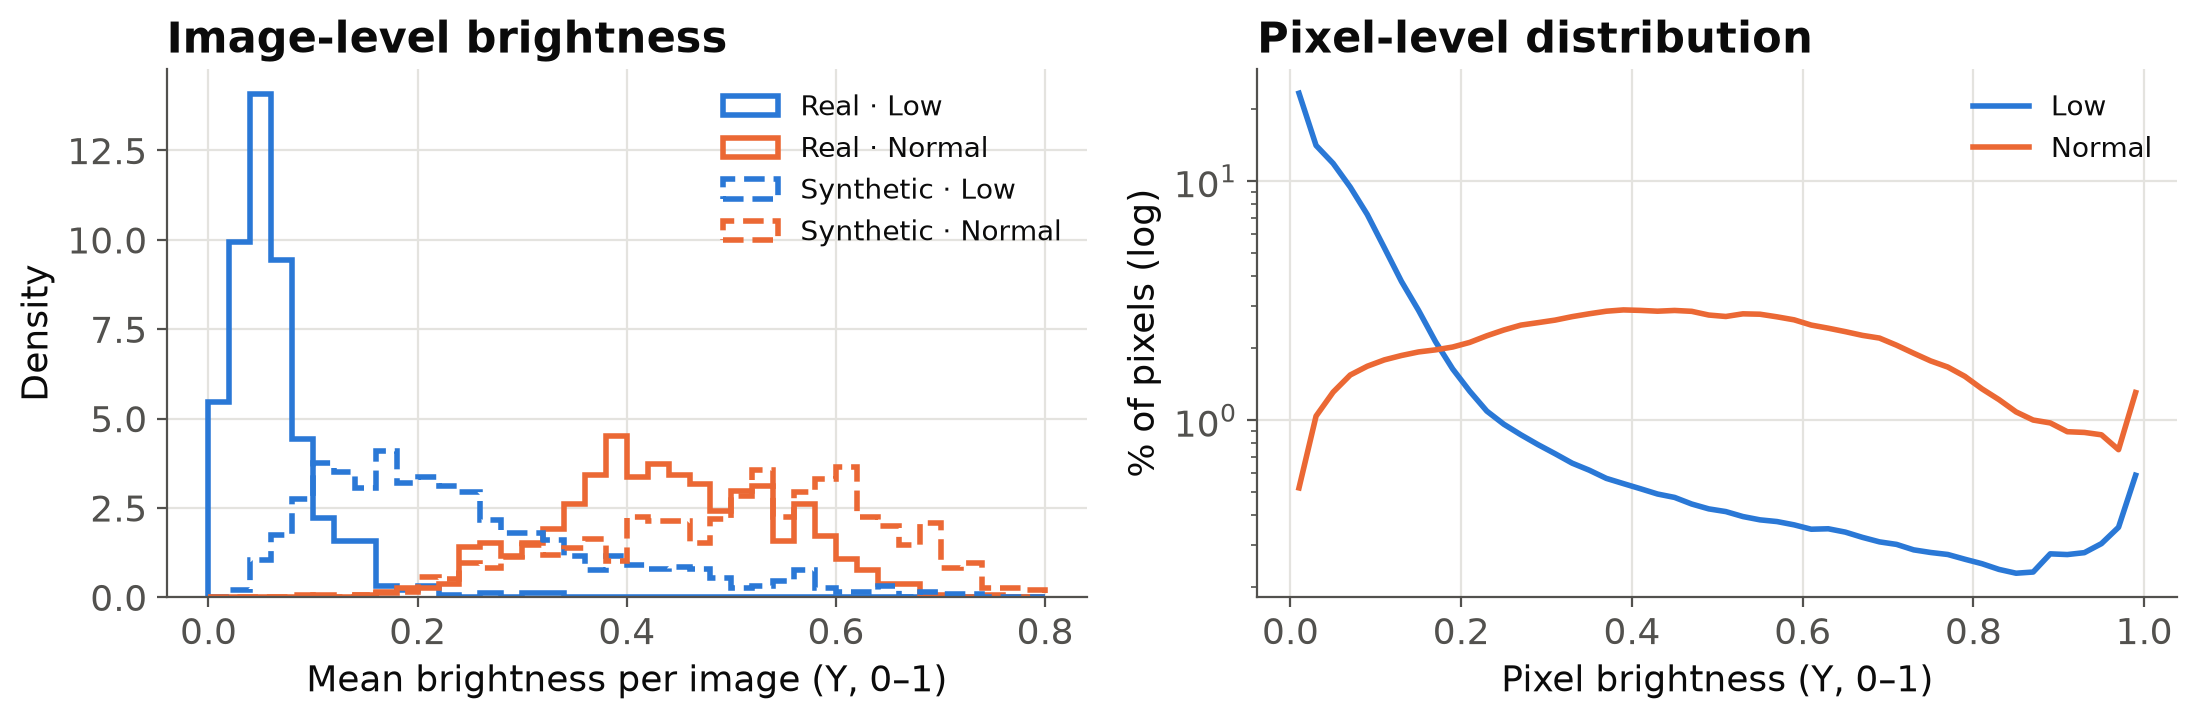
\includegraphics[width=\textwidth, height=0.52\textheight, keepaspectratio]{eda/brightness.png}
    \end{center}
    \vspace{-2mm}
    \begin{columns}[t]
        \begin{column}{0.5\textwidth}
            \footnotesize
            \textbf{Left:} real low-light images average $Y = 0.06$ vs.\ $0.44$ for GT; synthetic ones are much brighter ($0.24$) $\Rightarrow$ \textbf{real/synthetic domain gap}.
        \end{column}
        \begin{column}{0.5\textwidth}
            \footnotesize
            \textbf{Right:} 81\% of real low-light pixels have $Y < 0.1$ $\Rightarrow$ most information sits in a few dark grey levels, where noise dominates.
        \end{column}
    \end{columns}
\end{frame}

\begin{frame}
    \frametitle{Key EDA Insights (2/2): Brightening Is Not One Curve}
    \begin{columns}[c]
        \begin{column}{0.5\textwidth}
            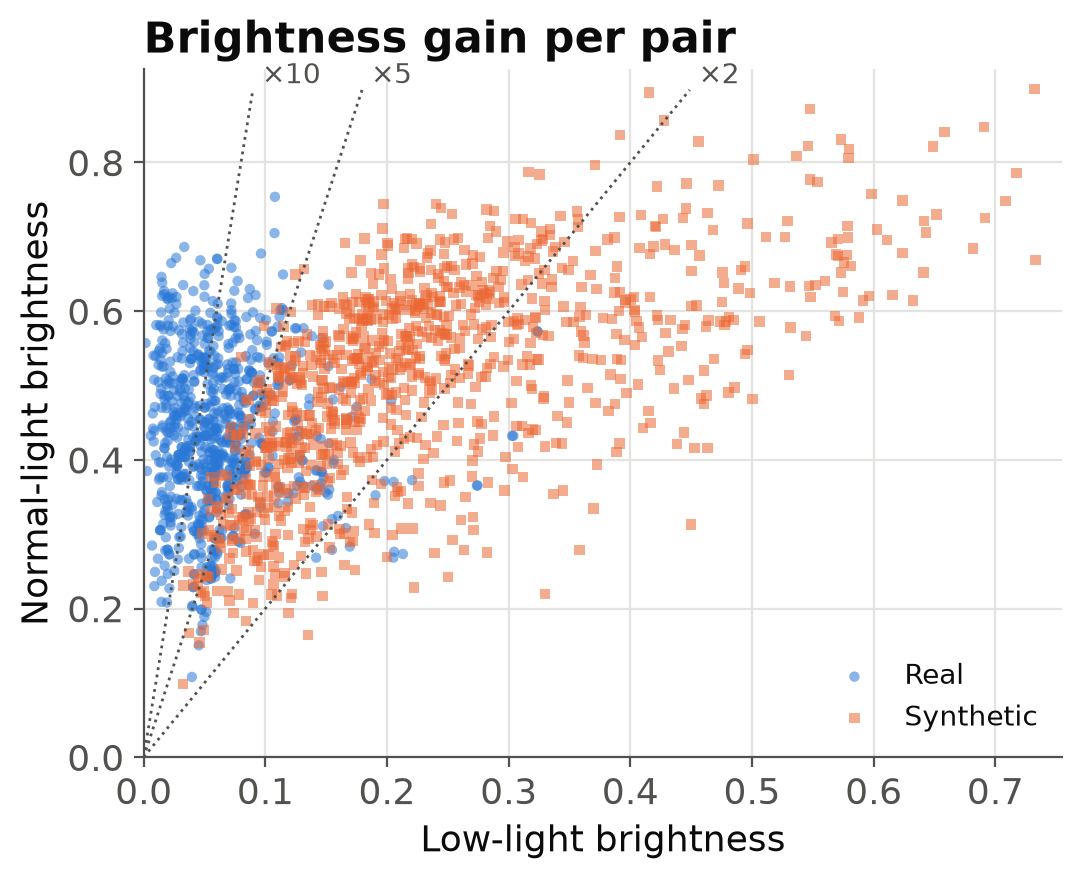
\includegraphics[width=\textwidth]{eda/gain_scatter.png}
        \end{column}
        \begin{column}{0.48\textwidth}
            \small
            Gain = GT brightness / low-light brightness
            \begin{itemize}
                \item Real: median $\times 7.5$, 90\% of pairs between $\times 2.8$ and $\times 30$.
                \item Synthetic: median $\times 2.5$ ($\times 1.1$ -- $\times 4.8$).
            \end{itemize}
            \vspace{2mm}
            \textbf{Conclusion:} the required brightening changes from image to image, so a global curve (gamma, histogram equalisation) cannot fit all pairs $\Rightarrow$ the model must learn \emph{content-aware} enhancement.
        \end{column}
    \end{columns}
\end{frame}
